%% GENERATED from paper_e_template.tex by docs/reports/paper_e/scripts/build_paper_e.py.
%% Do not edit: change the template and rebuild.
%% Paper E -- Computacion y Sistemas (CyS) template: cys.cls, cys.bst.
%% SOURCE FILE. paper_e.tex is generated from this file by scripts/build_paper_e.py, which
%% replaces every double-angle placeholder with a value read from outputs/analysis/paper_e/.
%% Do not type a result by hand.
%%
%% Review is blind: the default build omits author identity and the repository address.
%% The full build defines \fullversion before this file is read.
\documentclass{cys}

% The class asks for Helvetica (the journal's Arial). Under XeTeX (Tectonic) that needs fontspec.
\usepackage{iftex}
\ifPDFTeX
  \usepackage[utf8]{inputenc}
\else
  \usepackage{fontspec}
  \setmainfont{texgyreheros}[Extension=.otf,UprightFont=*-regular,BoldFont=*-bold,
    ItalicFont=*-italic,BoldItalicFont=*-bolditalic]
  \setsansfont{texgyreheros}[Extension=.otf,UprightFont=*-regular,BoldFont=*-bold,
    ItalicFont=*-italic,BoldItalicFont=*-bolditalic]
\fi
\usepackage[english]{babel}
\usepackage{graphicx}
\usepackage{amsmath}
\usepackage{url}
\usepackage{cite}
% Clickable citations, cross-references and URLs, in blue (author decision 2026-10-04).
% cys.cls does not load hyperref; published CyS articles that have links add it themselves.
% Loaded last. The PDF metadata carries no author, so the blind file stays blind.
\usepackage[colorlinks=true,allcolors=blue,pdfauthor={},pdfcreator={},pdfproducer={}]{hyperref}

\addto\captionsenglish{%
  \renewcommand{\figurename}{Fig.}%
  \renewcommand{\abstractname}{Abstract.}%
}
\setlength{\emergencystretch}{3em}
%% Paper E layout constants. Kept out of paper_e.tex because that file is under
%% [coverage] in pub/claim_registry.toml, where every decimal must be a registered result.
\newcommand{\tablestretch}{1.1}
\newlength{\tightcolsep}\setlength{\tightcolsep}{2.2pt}
\newlength{\mediumcolsep}\setlength{\mediumcolsep}{3pt}

%% Code and data archive (full version only). Set after the GitHub release is archived by
%% Zenodo; see README.md, "Release and archive".
\newcommand{\papererelease}{paper-e-cys-2026-10-04-r2}
\newcommand{\paperearchive}{\url{https://doi.org/10.5281/zenodo.23142429}}


\newif\iffull
\ifdefined\fullversion \fulltrue \else \fullfalse \fi

\title{Do Explainers Agree on Which Features Matter? \\ Instance-Level Agreement between SHAP and LIME}

\iffull
\author{Jonathan Herrera-V\'asquez$^{*}$}
\affil{
Universidad Americana de Europa (UNADE), Department of Computer Science, Canc\'un, \authorcr
Mexico
\authorcr \authorcr
jonnabio@gmail.com
\authorcr \authorcr
}
\else
\author{Author information omitted for blind review}
\affil{\authorcr}
\fi

\begin{document}

\maketitle

\renewcommand{\tablename}{Table}

\begin{abstract}
Post-hoc explainers are often used as if they were interchangeable, yet two explainers may
name different features for the same prediction. This study measures how much SHAP and LIME
agree at the level of the single instance. Both methods explained the same instances of
the same models on three tabular datasets (Adult, German Credit and Breast Cancer
Wisconsin), giving 31,411 paired explanations in 86 runs; LIME was
used with a fixed kernel width and without discretisation. The
analysis plan was written and committed before any agreement statistic was computed; runs,
not instances, are the unit of summary. The mean overlap of the five most important
features (Jaccard index) was 0.393 on Adult,
0.387 on German Credit and
0.714 on Breast Cancer. Part of this overlap does
not depend on the instance: the SHAP list of one instance and the LIME list of another
instance of the same run overlapped by 0.203,
0.287 and 0.648 (post hoc), so
the part specific to the instance was largest on Adult and smallest on Breast Cancer. A
post hoc experiment shows that neither method fully reproduces its own list when it is run again: on Adult the
overlap between two runs was 0.690 for LIME
and 0.782 for SHAP. Agreement between the methods was below this self-agreement for every model tested, so part of the disagreement is
variability of each method and part is a difference between them. Agreement varied between
models and datasets, did not vary visibly with the number of explained instances, and was
not consistently lower for misclassified instances. The agreement of signs was low and
followed the predicted class, because LIME without discretisation returns local slopes
while SHAP returns signed contributions; after conversion to contributions (post hoc), the
signs of the shared top features agreed in 0.945 to
0.990 of the cases, a level that one fixed direction per
feature also reaches.
\end{abstract}

\begin{keywords}
Explainable artificial intelligence, post-hoc explanations, disagreement problem, feature attribution, SHAP, LIME.
\end{keywords}

\section{Introduction}
\label{sec:introduction}

Post-hoc explanation methods describe a prediction of a trained model in terms of its input
features. SHAP \cite{lundberg2017unified} and LIME \cite{ribeiro2016why} are the most used
for tabular data: each returns, for one instance, a signed weight per feature. In practice
the two are treated as alternatives, and the choice between them is made on cost or habit.
That practice assumes that the explanation a user sees does not depend much on the method.

The assumption has been questioned. Krishna et al. \cite{krishna2024disagreement} named
the \emph{disagreement problem}: explanation methods often identify different top
features for the same prediction, and practitioners have no principled way to resolve the
conflict. Similar observations were made for text models \cite{neely2021order} and for
defect prediction \cite{roy2022why}. If the features shown to a user change with the
explainer, an explanation is a property of the pair (model, explainer), not of the model
alone, and conclusions drawn from it need the same caution
\cite{rudin2019stop,doshivelez2017rigorous}.

Most evidence on disagreement comes from a small number of models per dataset and treats
the explained instances as independent observations. Two points remain open for tabular
classifiers. The first is how much agreement varies with the model family, the dataset
and the number of explained instances when the same instances are explained by both
methods. The second is whether disagreement is related to two properties that
practitioners care about: whether the prediction is correct, and how good each
explanation is by the usual quality measures.

This study addresses both points with instance-paired explanations from an existing
benchmark cohort and a new, instance-aligned cohort produced for this purpose. The
research questions are:

\begin{itemize}
\item \textbf{RQ1.} For the same instance and model, how much do SHAP and LIME agree on
the most influential features and on their order?
\item \textbf{RQ2.} How does this agreement vary with the model family, the sampling
intensity and the dataset?
\item \textbf{RQ3.} Is agreement different for correctly classified and misclassified
instances?
\item \textbf{RQ4.} Is disagreement on an instance associated with the fidelity or the
stability of either explanation?
\end{itemize}

A secondary, descriptive question is how the features used by two explainers of a
different kind, Anchors \cite{ribeiro2018anchors} and DiCE \cite{mothilal2020dice},
overlap with those of SHAP and LIME.

The contributions are: (i) estimates of SHAP--LIME agreement on 31,411 paired
explanations across five model families and three datasets, with the run as the unit of
summary; (ii) two references that earlier comparisons lack (post hoc): the overlap between
explanations of different instances, which isolates the agreement that depends on the
instance, and the
agreement of each method with itself when it is run again, which separates the variability
of a method from the difference between methods; (iii) evidence that agreement varies between
models and datasets, not visibly with the number of explained instances, and is not
consistently related to prediction correctness, also when training instances are
excluded (post hoc); (iv) an association between disagreement and the fidelity of the LIME
explanation on two datasets; and (v) a methodological finding (post hoc): the sign
agreement between SHAP and LIME without discretisation is determined mostly by the
predicted class, because the two methods return different quantities.

\section{Related Work}
\label{sec:related}

\textbf{Disagreement between explainers.} Krishna et al. \cite{krishna2024disagreement}
formalised disagreement with measures of feature agreement, rank agreement, sign
agreement and rank correlation over the top-$k$ features, and reported frequent
disagreement across datasets and models, together with interviews showing that
practitioners resolve it with ad hoc rules. Neely et al. \cite{neely2021order} found low
rank correlation between attribution methods for text classifiers and argued that
agreement should not be used to validate a method. Roy et al. \cite{roy2022why}
compared LIME and SHAP on defect prediction models with measures of feature, rank and
sign agreement, and reported that the two methods disagree, more often on the rank of the
features than on their sign.

\textbf{Why methods differ.} Han et al. \cite{han2022which} showed that several
attribution methods are local function approximations of the model that differ in the
neighbourhood and the loss they use, so that no method is best for every neighbourhood.
Garreau and von Luxburg \cite{garreau2020explaining} analysed LIME for tabular data in
its default form, which discretises the features, and showed that, for a linear model, its
coefficients are proportional to the gradient of the model. SHAP values, in contrast, distribute the difference between the prediction and
an expected prediction among the features \cite{lundberg2017unified,lundberg2020local}.
This difference of meaning matters for the sign analysis in
Section~\ref{sec:results:sign}.

\textbf{Reliability of explanations.} Explanations can change under small perturbations
of the input \cite{alvarezmelis2018robustness} and can be manipulated
\cite{slack2020fooling}. Stability and fidelity are therefore common quality criteria.
This study relates them to disagreement at the level of the instance, which, to the author's knowledge, earlier work on tabular data has not reported with a
clustered design.

\section{Materials and Methods}
\label{sec:methods}

\subsection{Datasets, Models and Runs}

Three public binary classification datasets were used: Adult \cite{becker1996adult}
(108 encoded features), German Credit \cite{hofmann1994statlog} (61 encoded features) and
Breast Cancer Wisconsin, diagnostic \cite{wolberg1993breast} (30 numeric features).
Numeric features were standardised and categorical features were one-hot encoded; each
encoded column is one feature in every analysis.

On Adult, five model families were explained: logistic regression (LR), a support
vector machine with probability outputs (SVM), a multilayer perceptron (MLP), a random
forest (RF) \cite{breiman2001random} and gradient boosting (XGB) \cite{chen2016xgboost}.
Each explainer was run with five random seeds and three sampling intensities
($n = 50$, $100$ and $200$ test instances per quadrant of the confusion matrix), so that
correct and incorrect predictions are both represented. Each Adult model was trained once, on the partition of the data given by seed 42; the
seed of a run fixes the partition from which its instances are drawn. For the four seeds
other than 42 that partition differs from the one used in training, so part of the
explained instances belong to the training data of the model. On German Credit and Breast
Cancer, RF and XGB models were trained with three seeds each, on the partition of the same
seed, and explained with one intensity (up to 100 instances per quadrant).

\iffull
The Adult runs and the SHAP and Anchors runs of the other two datasets belong to a
benchmark cohort described in \cite{herrera2026framework}. That work compares explainers
by quality measures; no result of it is repeated here.
\else
The Adult runs and the SHAP and Anchors runs of the other two datasets belong to a
benchmark cohort described in an earlier publication (reference withheld for blind
review). That work compares explainers by quality measures; no result of it is repeated
here.
\fi
Two companion manuscripts use the same cohort: one proposes a taxonomy of evaluation
metrics and compares LIME and SHAP by quality measures, and the other studies explanation
quality on correct and incorrect predictions. Neither studies agreement between
explainers, and no result of either is repeated here.

The earlier LIME runs on German Credit and Breast Cancer explained a different sample of
instances and stored only averages. \emph{A new LIME cohort was therefore produced for
this study}: for each dataset, model and seed, LIME explained exactly the instances
stored in the corresponding SHAP run. The model binaries were regenerated from the
training recipe in the repository, and the run was allowed only after the regenerated
model reproduced the stored training metrics, the feature order and the stored label and
prediction of every target instance.

\subsection{Explainers}
\label{sec:methods:explainers}

\textbf{SHAP.} TreeSHAP \cite{lundberg2020local} was used for RF and XGB, in its
interventional form and on the probability scale, and KernelSHAP
\cite{lundberg2017unified} for LR, SVM and MLP, both with 50 background instances drawn
from the training data. The stored value of a feature is its signed contribution to the
predicted probability of class~1, relative to the expected probability on the background
data.

\textbf{LIME.} The tabular explainer \cite{ribeiro2016why} was used with 1000 perturbed
samples, kernel width 3, ten selected features and \emph{without discretisation of
continuous features}. The kernel width was the same for the three datasets; it is smaller
than the default of the package, three quarters of the square root of the number of
features (between about four and eight here). With these settings, LIME draws its perturbed samples from a normal distribution
with the mean and the standard deviation of the training data, weights them by their
distance to the instance, and standardises each feature; all encoded columns, including
the one-hot columns, are treated as continuous. It first fits a linear model on all
features and keeps the ten with the largest product of coefficient and standardised value
of the instance, and then fits the final model on those ten. The stored value of a
feature is its coefficient in that final model for the probability of class~1, that is, a
slope on the standardised scale. The ten LIME features are therefore selected by the size
of their contribution and ordered, in the stored list, by the size of their slope.

\textbf{Anchors and DiCE} (Adult, secondary analysis). Anchors
\cite{ribeiro2018anchors} returns a rule; its feature set is the set of features in the
rule. DiCE \cite{mothilal2020dice} returns counterfactual instances; its feature set is
the set of features whose value changes. Neither is a signed attribution, so only
feature sets are compared.

For each instance, a run stores the ten features with the largest absolute value, in
that order (for LIME, the ten selected features). All measures below use these stored
lists.

\subsection{Agreement Measures}

Let $S_k$ and $L_k$ be the sets of the $k$ features with the largest absolute SHAP and
LIME values for one instance. The primary measure is the top-5 Jaccard overlap
\cite{jaccard1912distribution}:
\begin{equation}
J_5 = \frac{|S_5 \cap L_5|}{|S_5 \cup L_5|}.
\label{eq:jaccard}
\end{equation}
Three shared features out of five give $J_5 = 3/7$, and four give $J_5 = 4/6$. The top-10 overlap $J_{10}$ is a sensitivity measure.

Rank concordance is Kendall's $\tau_b$ \cite{kendall1945treatment} computed on the union
of the two top-10 lists; a feature absent from a list receives rank 11, and ties use
midranks. A feature present in only one list lowers this coefficient, so the measure
combines the overlap of the lists with the order within them, and zero is not its value
for unrelated orders. As a sensitivity analysis (post hoc), $\tau_b$ was also computed on
the features present in both lists only.

Sign agreement is the fraction of the features in $S_5 \cap L_5$, with both values
different from zero, whose SHAP and LIME values have the same sign. For the post hoc
analysis of Section~\ref{sec:results:sign}, the LIME slope $w_j$ of feature $j$ was
converted into a contribution relative to the training mean $m_j$:
\begin{equation}
c_j = w_j \, \frac{x_j - m_j}{s_j},
\label{eq:contribution}
\end{equation}
where $x_j$ is the value of the feature for the instance and $s_j$ the standard deviation
used by LIME. This is the term of feature $j$ in the local linear model of LIME, so
$c_j$ and the SHAP value are both contributions relative to a reference. The sign
agreement was then recomputed with the sign of $c_j$.

Three references for the overlap were added post hoc. The first is the expected
value of $J_k$ for two independent random sets of $k$ features out of $p$, computed exactly
from the hypergeometric distribution. For $k = 5$ it is 0.026 on Adult,
0.047 on German Credit and 0.099 on Breast
Cancer. The second is a \emph{permutation reference}: within each run, the SHAP list of
every instance was compared with the LIME list of another instance of the same run, drawn
at random (20 draws per instance). It measures the overlap that comes from a ranking of
the features common to the instances of a run; the paired overlap minus this value is the
\emph{instance-specific part}. The third is the \emph{self-agreement} of each method: a subsample of
the paired instances (20 per run on Adult at $n = 100$ and 30 per run on the other datasets) was explained twice by LIME and twice by SHAP with the settings of
the stored runs, the two repetitions differing only in the random state (the perturbed
samples of LIME; the background sample of SHAP and the coalition sampling of KernelSHAP).
The same measures were computed between the two repetitions, between the new SHAP and
LIME runs and, as the permutation reference of this experiment, between every instance and
the other instances of its run. Each instance was also explained twice by LIME with the
default kernel width, all other settings unchanged. An instance entered only if the loaded
model reproduced its stored prediction; this excluded 32 candidates of the Adult
random forest, whose stored binary does not reproduce all the recorded predictions, and
none of the other models. The SVM was left out, because KernelSHAP on it is too slow for repeated runs and its stored runs are incomplete.

\subsection{Pairing and Quality Control}

Explanations were paired by dataset, model, seed, intensity and instance identifier.
Only instances with a valid explanation from both methods and the same stored label and
prediction entered the analysis. The source runs contained 278 records
with an error and no explanation, mostly KernelSHAP on the SVM; these were excluded,
and one SVM block had no usable SHAP run. The SHAP runs of the SVM are incomplete: they
hold explanations for 2,064 of the
7,000 instances explained by LIME
(29.5\%), and these are not balanced between the
predicted classes. The SVM estimates rest on this subset and are less reliable than those
of the other families, whose coverage is complete. Of the 87 blocks, 76
had identical sets of valid instances for the two methods; in the others the
intersection was used, which left 4,936 valid records unpaired. No paired
record had a different label or prediction in the two runs. The result is 31,411
paired explanations in 86 runs: 29,667 on Adult
(74 runs), 1,060 on German Credit and
684 on Breast Cancer (six runs each). Kendall's $\tau_b$ was
undefined for 0 pairs and sign agreement for 516 pairs
without a shared non-zero feature.

\subsection{Statistical Summary}
\label{sec:methods:stats}

The same test instances recur across models, seeds and intensities, so instances are not
independent replicates. Each measure was first averaged within a run (dataset, model,
seed, intensity). The point estimate of a group is the mean of its run means. The 95\%
interval is a percentile bootstrap with 2000 resamples in which random seeds, not
instances, are resampled with replacement, and all runs of a sampled seed are kept
together \cite{efron1993introduction,cameron2015practitioner}. There are five seeds on
Adult and three on the other datasets. With three seeds the limits of this interval are
the smallest and the largest seed mean, and with five they are close to them; the
intervals are therefore reported as a description of the variation between seeds, not as
intervals with a known coverage, and they are not used as tests. On Adult each model
family is one fitted model, so its interval reflects the partition, the sampled instances
and the randomness of the explainers, not the variation between fits.

For RQ3, the difference between the mean $J_5$ of misclassified and of correctly
classified instances was computed within each run that had at least ten instances in
each group, averaged over intensities for each model and seed, and summarised by model.
On Adult the contrast was repeated (post hoc) on the instances that are not rows of the
training data of the model.

For RQ4, the Spearman correlation between disagreement ($1 - J_5$) and each of four
quality values of the instance (fidelity and stability of the SHAP and of the LIME
explanation) was computed within each run and averaged by seed. Fidelity, a single-feature variant of the faithfulness measure of
\cite{bhatt2020evaluating}, is the Pearson correlation, across features, between the
absolute value of the attribution and the absolute change in the predicted probability
when that feature alone is replaced by its training mean. Stability, in the spirit of \cite{alvarezmelis2018robustness}, is the mean pairwise
cosine similarity between the explanations of 15 copies of the instance with small
Gaussian noise added to every encoded column. Both were
computed and stored with each explanation when the runs were made.

No hypothesis test was planned and no $p$-value is reported. The estimates for RQ2 to RQ4
are exploratory.

\subsection{Pre-specification and Deviations}

The analysis plan, with the measures, the unit of analysis, the exclusion rules and the
bootstrap settings, was written and committed to the project repository before any
agreement statistic was computed and before the new LIME cohort was run. It is a
time-stamped commit in the author's repository\iffull{} (\texttt{7726bb0a9})\fi, not an entry in an independent registry.
Two refinements made before the analysis are recorded in the plan. The plan assumed that
SHAP and LIME both return signed contributions; for LIME as configured this was wrong,
which the analysis of signs revealed.

The following analyses are \emph{post hoc}, were added after the planned results were
inspected or in response to an independent review of the manuscript, and are recorded in
the plan as dated deviations: the three references for the overlap (chance, permutation
and self-agreement), with the repetition of LIME at the default kernel width and the
description of the kernel weights and of the stored LIME stability; the breakdown of sign agreement by predicted class, the constancy of the
sign of each feature, and the conversion of the LIME slopes into contributions with its
baseline (Section~\ref{sec:results:sign}); the two sensitivity analyses of the rank
measure; and the correctness contrast on held-out instances. The feature values needed for
the conversion were reloaded with the code that produced the runs; the stored label of
every paired instance matched the reloaded data.

\section{Results}
\label{sec:results}

\subsection{Agreement on the Top Features (RQ1)}

Table~\ref{tab:agreement} and Fig.~\ref{fig:overlap} give the agreement estimates. On
Adult, the mean top-5 overlap was 0.393 (95\%
interval 0.377 to
0.410); on German Credit it was
0.387 (0.343
to 0.426). The mean number of shared features with a non-zero value in both
lists was 2.70 and 2.67 out
of five. On Breast Cancer the overlap was
0.714 (0.671
to 0.792), with 4.05 shared features on average. The medians of the run means were
0.393, 0.416 and
0.712. In all three datasets the
overlap was several times the expected overlap of random sets.

A large part of the overlap, however, does not depend on the instance (post hoc;
Table~\ref{tab:agreement}, column Other). The SHAP list of an instance and the LIME list
of another instance of the same run overlapped by 0.203 on
Adult, 0.287 on German Credit and
0.648 on Breast Cancer. The instance-specific part was thus
0.191 on Adult (0.184 to
0.195), 0.100 on German
Credit and 0.066 on Breast Cancer, and it was positive in
every run. Most of the high overlap on Breast Cancer is thus agreement on a ranking common
to the instances; the instance-specific part was largest on Adult.

The rank measure, which combines overlap and order, was low on two datasets. Kendall's
$\tau_b$ was
0.126 on Adult and
0.122 on German Credit, and
0.517 on Breast Cancer. Extending the lists to
ten features raised the overlap on Adult and German Credit
(0.507 and
0.480) and lowered it slightly on Breast Cancer
(0.669). Restricted to the features present in
both top-10 lists, $\tau_b$ was 0.193,
0.243 and
0.613: the order of the shared features is
positively but weakly related on Adult and German Credit.

Because LIME orders its ten features by slope and SHAP by contribution
(Section~\ref{sec:methods:explainers}), the LIME lists were also re-ordered by the absolute
contribution of Eq.~(\ref{eq:contribution}). The top-5 overlap was then
0.416 on Adult,
0.393 on German Credit and
0.633 on Breast Cancer, close to the planned
estimates on the first two and lower on the third. The low overlap is thus not produced
by ordering slopes against contributions.

\subsection{Agreement of Each Method with Itself (Post Hoc)}
\label{sec:results:ceiling}

Table~\ref{tab:ceiling} gives the overlap between two runs of the same method on the same
instances and the SHAP--LIME overlap between the new runs, each with its permutation
reference. Neither method reproduced its own top-5 list. On Adult the overlap between two LIME runs
was 0.690 and between two SHAP runs
0.782; on German Credit
0.642 and
0.708; on Breast Cancer
0.836 and
0.939. The SHAP--LIME overlap was below
the self-agreement of both methods for every model in the table. This holds between the
new runs (Adult: 0.383; its random forest: 0.353)
as between the stored explanations of the same instances (0.393 and
0.356).

The permutation reference shows that the same holds for the instance-specific part. On
Adult, explanations of different instances overlapped by 0.195 for two
LIME runs, 0.376 for two SHAP runs and 0.209
for SHAP and LIME, so each method is far more specific to the instance with itself than
with the other method. On Breast Cancer the overlap between different instances is high
for all three
(0.709, 0.675 and 0.659),
so a large part of the self-agreement, like most of the agreement between the methods,
belongs there to a ranking common to the instances.

Two consequences follow. First, identity is not the right upper reference for agreement
between the methods: a second run of LIME, with 1000 perturbed samples for up to 108
features, already changes part of the list, and so does a second run of SHAP with another
background sample of 50 instances. Second, self-agreement differs between models: the
multilayer perceptron had the lowest self-agreement of LIME and the lowest SHAP--LIME
overlap, but the other three Adult models show no such relation. The
subsample is small and the experiment was not planned; it bounds the question and does not
give a precise decomposition.

\textbf{Kernel width.} The experiment was repeated for LIME with the default kernel
width. Its lists changed: on Adult the top-5 overlap between LIME at width 3 and LIME at
the default width was 0.370, as low as between SHAP and LIME; it was
0.590 on German Credit and 0.889 on Breast Cancer. The
overlap of SHAP with default-width LIME was higher on Adult (0.456
against 0.383), with models moving in both directions (from
0.353 to 0.533 for the random forest,
from 0.346 to 0.286 for the
multilayer perceptron), and about the same on the other two datasets. Default-width LIME
was also less specific to the instance: on Adult two of its explanations of different
instances overlapped by 0.589, against 0.195 at
width 3. The kernel width thus changes the LIME explanation as much as the change of
explainer does, and the narrow kernel gives the explanations that depend more on the
instance.


\begin{table*}[t]
\renewcommand{\arraystretch}{\tablestretch}
\centering
\caption{Agreement between SHAP and LIME: mean of run means and seed-clustered 95\% interval (the spread of the seed means, Section~\ref{sec:methods:stats}). Other: top-5 overlap of the SHAP list of an instance with the LIME list of another instance of the same run (post hoc). Adult rows pool the three sampling intensities; the SVM row rests on 29.5\% of its instances}
\label{tab:agreement}
\small
\setlength{\tabcolsep}{\mediumcolsep}
\begin{tabular}{llrrlrll}
\hline
Dataset & Model & Runs & Pairs & Top-5 Jaccard & Other & Top-10 Jaccard & Kendall $\tau_b$ \\
\hline
% GENERATED by scripts/build_paper_e.py -- do not edit
Adult & LR & 15 & 7,000 & 0.485 [0.464, 0.505] & 0.261 & 0.617 [0.584, 0.640] & 0.263 [0.221, 0.304] \\
 & SVM & 14 & 2,064 & 0.395 [0.388, 0.404] & 0.206 & 0.516 [0.489, 0.539] & 0.171 [0.148, 0.187] \\
 & MLP & 15 & 7,000 & 0.335 [0.326, 0.341] & 0.128 & 0.441 [0.435, 0.448] & 0.043 [0.029, 0.054] \\
 & RF & 15 & 6,603 & 0.389 [0.360, 0.415] & 0.199 & 0.560 [0.530, 0.590] & 0.129 [0.090, 0.168] \\
 & XGB & 15 & 7,000 & 0.363 [0.328, 0.399] & 0.219 & 0.404 [0.384, 0.422] & 0.028 [$-$0.020, 0.071] \\
 & All & 74 & 29,667 & 0.393 [0.377, 0.410] & 0.203 & 0.507 [0.487, 0.525] & 0.126 [0.100, 0.153] \\
\hline
German Credit & RF & 3 & 523 & 0.464 [0.450, 0.471] & 0.339 & 0.542 [0.519, 0.572] & 0.237 [0.212, 0.251] \\
 & XGB & 3 & 537 & 0.309 [0.235, 0.381] & 0.235 & 0.419 [0.395, 0.440] & 0.008 [$-$0.101, 0.096] \\
 & All & 6 & 1,060 & 0.387 [0.343, 0.426] & 0.287 & 0.480 [0.457, 0.506] & 0.122 [0.055, 0.172] \\
\hline
Breast Cancer & RF & 3 & 342 & 0.738 [0.678, 0.790] & 0.651 & 0.665 [0.643, 0.691] & 0.526 [0.494, 0.571] \\
 & XGB & 3 & 342 & 0.690 [0.612, 0.795] & 0.646 & 0.673 [0.666, 0.681] & 0.507 [0.457, 0.551] \\
 & All & 6 & 684 & 0.714 [0.671, 0.792] & 0.648 & 0.669 [0.654, 0.682] & 0.517 [0.475, 0.561] \\
\hline

\end{tabular}
\end{table*}

\begin{figure*}[t]
\centering
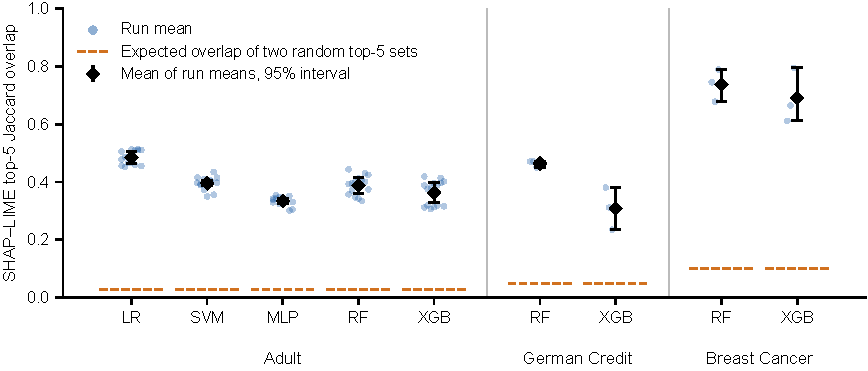
\includegraphics[width=\textwidth]{figures/fig1_top5_overlap.pdf}
\caption{Top-5 overlap between SHAP and LIME by dataset and model family. Each point is the mean of one run; intervals are the spread of the seed means}
\label{fig:overlap}
\end{figure*}

\begin{table*}[t]
\renewcommand{\arraystretch}{\tablestretch}
\centering
\caption{Top-5 Jaccard overlap between two runs of the same method with different random states, and between the new SHAP and LIME runs, on the same subsample of instances: mean of run means and seed-clustered interval (spread of the seed means). Other: the same pair between an instance and the other instances of its run. Post hoc}
\label{tab:ceiling}
\small
\setlength{\tabcolsep}{\mediumcolsep}
\begin{tabular}{llrlrlrlr}
\hline
 & & & \multicolumn{2}{c}{LIME vs. LIME} & \multicolumn{2}{c}{SHAP vs. SHAP} & \multicolumn{2}{c}{SHAP vs. LIME} \\
Dataset & Model & Inst. & Same instance & Other & Same instance & Other & Same instance & Other \\
\hline
% GENERATED by scripts/build_paper_e.py -- do not edit
Adult & LR & 100 & 0.774 [0.736, 0.806] & 0.759 [0.709, 0.804] & 0.494 [0.420, 0.575] \\
 & MLP & 100 & 0.526 [0.508, 0.549] & 0.728 [0.685, 0.780] & 0.338 [0.304, 0.371] \\
 & RF & 100 & 0.783 [0.755, 0.808] & 0.887 [0.840, 0.937] & 0.356 [0.311, 0.407] \\
 & XGB & 100 & 0.676 [0.636, 0.706] & 0.754 [0.709, 0.807] & 0.385 [0.331, 0.460] \\
 & All & 400 & 0.690 [0.670, 0.705] & 0.782 [0.743, 0.824] & 0.393 [0.347, 0.444] \\
\hline
German Credit & RF & 90 & 0.642 [0.621, 0.674] & 0.708 [0.689, 0.730] & 0.445 [0.438, 0.452] \\
 & XGB & 90 & 0.643 [0.609, 0.665] & 0.709 [0.660, 0.792] & 0.319 [0.254, 0.393] \\
 & All & 180 & 0.642 [0.615, 0.664] & 0.708 [0.682, 0.749] & 0.382 [0.349, 0.416] \\
\hline
Breast Cancer & RF & 90 & 0.825 [0.754, 0.937] & 0.952 [0.933, 0.967] & 0.747 [0.688, 0.837] \\
 & XGB & 90 & 0.847 [0.770, 0.956] & 0.927 [0.911, 0.948] & 0.701 [0.613, 0.821] \\
 & All & 180 & 0.836 [0.762, 0.946] & 0.939 [0.922, 0.957] & 0.724 [0.664, 0.829] \\
\hline

\end{tabular}
\end{table*}

\subsection{Model Family, Sampling Intensity and Dataset (RQ2)}

On Adult, agreement differed between the five fitted models. The overlap was highest for
logistic regression (0.485) and lowest for the
multilayer perceptron (0.335); the first was above
the second in each of the five seeds. The rank measure was lowest for the multilayer perceptron
(0.043) and for gradient boosting
(0.028). Each family is represented by one fitted
model, and the self-agreement of LIME was also lowest for the multilayer perceptron
(Table~\ref{tab:ceiling}), so these differences cannot be attributed to the model family
as such. On German Credit the overlap was higher for the random forest
(0.464) than for gradient boosting
(0.309); on Breast Cancer the two families were
close.

The sampling intensity had no visible effect: pooled over models, the top-5 overlap on
Adult was 0.395, 0.394 and
0.390 for 50, 100 and 200 instances per quadrant. 

The dataset changed the estimates most, but not in one direction. Adult and German
Credit, with many one-hot encoded features, gave similar and low overlap; Breast Cancer,
with 30 numeric features, gave much higher overlap for the same two model families. The
permutation reference reverses this order for the instance-specific part, which was
largest on Adult and smallest on Breast Cancer (Table~\ref{tab:agreement}). Two things
differ together between the datasets: the kind of features, and the weight that the fixed
kernel of LIME gives to its perturbed samples, which falls as the number of features grows
(Section~\ref{sec:discussion}). Three datasets do not allow the difference to be
attributed to either.

\subsection{Agreement of Signs (Post Hoc)}
\label{sec:results:sign}

The planned sign agreement on shared top-5 features was
0.717 on Adult
(0.687 to 0.747),
0.511 on German Credit
(0.481 to
0.528) and
0.374 on Breast Cancer
(0.357 to
0.385). It is defined on the shared features
only, whose mean number was given above. The last value is below
one half, on the dataset where the two methods agree most on which features matter. This
led to the post hoc analysis in Table~\ref{tab:sign} and Fig.~\ref{fig:sign}.

Sign agreement depended strongly on the predicted class. On Breast Cancer it was
0.977 for instances predicted as class~0 and
0.036 for instances predicted as class~1. On Adult it was
0.875 for class~1 and 0.506 for
class~0, and the same pattern appeared in four of the five model families; the
multilayer perceptron was the exception.

The reason is that the two methods return different quantities
(Section~\ref{sec:methods:explainers}). The LIME coefficient of a continuous feature is a
local slope. The slope of a feature with a monotone effect has the same sign for most
instances. A SHAP value is a contribution relative to the expected output: for the same
feature it is positive for instances on one side of the reference and negative on the
other. The two signs therefore coincide for the instances of one predicted class and
differ for the other. The constancy measure confirms it: on Breast Cancer, a feature
kept its majority sign in 0.993 of its LIME explanations
and in 0.621 of its SHAP explanations
(0.912 and 0.679 on German
Credit; 0.850 and 0.757 on
Adult, where most features are one-hot indicators).

The conversion of Eq.~(\ref{eq:contribution}) removes this difference. When each LIME
slope was converted into a contribution, the sign agreement rose to
0.945 on Adult (95\% interval
0.941 to 0.949),
0.960 on German Credit
(0.953 to 0.964) and
0.990 on Breast Cancer
(0.983 to 0.997), and the
dependence on the predicted class disappeared: on Breast Cancer it was
0.991 for class~0 and 0.989 for
class~1, and on Adult 0.927 and
0.958. It exceeded nine tenths for every model family
(Table~\ref{tab:sign}).

This high value must be read with its baseline. The conversion multiplies the slope by
the deviation of the feature from its mean, and the sign of a SHAP value for a feature
with a monotone effect carries the same factor. What is left to agree is one direction
per feature. A baseline that uses no instance-level information from LIME shows this:
when the sign of every LIME slope was replaced by the majority sign of that feature in
the same run, the agreement with SHAP after conversion was
0.951 on Adult, 0.978 on
German Credit and 0.990 on Breast Cancer, as high as with
the slopes of each instance.

Sign agreement between SHAP and LIME without discretisation is thus not a measure of
disagreement about the direction of an effect; it measures mostly on which side of the
reference the instance lies. After conversion, the two methods imply the same direction
for nearly all the features that both place among the five most important, and this
direction is a global one per feature. The result does not show that the two methods
agree on instance-specific directions, which these data cannot test.

\begin{table}[t]
\renewcommand{\arraystretch}{\tablestretch}
\centering
\caption{Sign agreement on shared top-5 features, overall and by predicted class (Cl.), with the LIME value as stored (slope) and after conversion into a contribution. The column All of the slope block is the prespecified estimate; the rest is post hoc}
\label{tab:sign}
\footnotesize
\setlength{\tabcolsep}{\tightcolsep}
\begin{tabular}{llrrrrrr}
\hline
 & & \multicolumn{3}{c}{Slope} & \multicolumn{3}{c}{Contribution} \\
Dataset & Model & All & Cl.~0 & Cl.~1 & All & Cl.~0 & Cl.~1 \\
\hline
% GENERATED by scripts/build_paper_e.py -- do not edit
Adult & LR & 0.696 & 0.527 & 0.864 & 0.947 & 0.947 & 0.948 \\
 & SVM & 0.829 & 0.332 & 0.956 & 0.952 & 0.918 & 0.960 \\
 & MLP & 0.689 & 0.706 & 0.672 & 0.951 & 0.940 & 0.962 \\
 & RF & 0.696 & 0.418 & 0.975 & 0.948 & 0.913 & 0.984 \\
 & XGB & 0.682 & 0.443 & 0.916 & 0.925 & 0.911 & 0.939 \\
 & All & 0.717 & 0.506 & 0.875 & 0.945 & 0.927 & 0.958 \\
\hline
German Credit & RF & 0.470 & 0.608 & 0.430 & 0.985 & 0.990 & 0.983 \\
 & XGB & 0.553 & 0.716 & 0.494 & 0.934 & 0.933 & 0.934 \\
 & All & 0.511 & 0.662 & 0.462 & 0.960 & 0.962 & 0.959 \\
\hline
Breast Cancer & RF & 0.377 & 0.975 & 0.041 & 0.997 & 1.000 & 0.995 \\
 & XGB & 0.371 & 0.979 & 0.032 & 0.983 & 0.983 & 0.983 \\
 & All & 0.374 & 0.977 & 0.036 & 0.990 & 0.991 & 0.989 \\
\hline

\end{tabular}
\end{table}

\begin{figure*}[t]
\centering
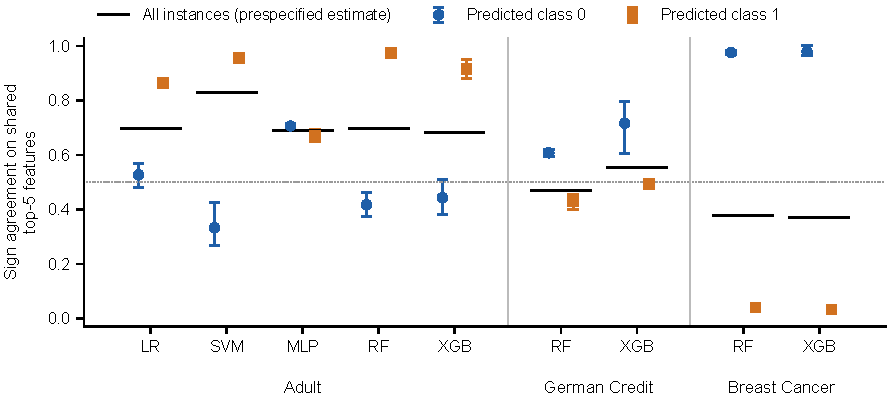
\includegraphics[width=\textwidth]{figures/fig2_sign_by_class.pdf}
\caption{Sign agreement between SHAP and LIME. Circles and squares: LIME value as stored (slope), by predicted class, with seed-clustered 95\% intervals (spread of the seed means). Diamonds: all instances after the slopes were converted into contributions. The dotted line marks one half}
\label{fig:sign}
\end{figure*}

\subsection{Correct and Misclassified Instances (RQ3)}

Table~\ref{tab:correctness} and Fig.~\ref{fig:correctness} give the difference in top-5
overlap between misclassified and correctly classified instances. The direction was not
consistent. For the multilayer perceptron, agreement was lower on misclassified
instances (difference $-$0.059, interval
$-$0.069 to $-$0.049, same direction in all five
seeds). For the random forest it was higher (0.045,
0.029 to 0.064, all five seeds), and slightly
higher for gradient boosting (0.014). For logistic regression and
the support vector machine the difference was near zero. On German Credit the
differences were small and negative, with three seeds. On Breast Cancer no run had ten
misclassified instances, so the contrast could not be estimated. The largest difference
in absolute value was that of the multilayer perceptron, small compared with the
differences between models.

On Adult this contrast is entangled with membership in the training data. For the four
seeds other than 42, 0.707 of the paired
instances are rows of the training data, and for the random forest
0.840 of the correctly classified
instances are training rows against 0.006
of the misclassified ones. The contrast was therefore repeated on held-out instances
only. The pattern remained: for the multilayer perceptron the difference was
$-$0.042 ($-$0.058 to
$-$0.024, negative in all five seeds), for the random forest
0.049 (0.032 to
0.066, positive in all five seeds), and for logistic regression and
gradient boosting 0.000 and
$-$0.004, with seeds of both signs. For the support
vector machine only 5 of 14 runs had ten
held-out instances in each group; the difference was
0.028, with seeds of both signs. The differences
of the multilayer perceptron and the random forest are thus not produced by the training instances, and their opposite
signs remain.

\begin{table}[t]
\renewcommand{\arraystretch}{\tablestretch}
\centering
\caption{Top-5 overlap for correctly classified (C) and misclassified (M) instances. Diff.\ is M minus C, with the spread of the seed means; Neg.\ is the number of seeds with a negative difference; GC is German Credit. The SVM row rests on incomplete runs}
\label{tab:correctness}
\footnotesize
\setlength{\tabcolsep}{\tightcolsep}
\begin{tabular}{llrrrlr}
\hline
Data & Model & C & M & Diff. & 95\% interval & Neg. \\
\hline
% GENERATED by scripts/build_paper_e.py -- do not edit
Adult & LR & 0.486 & 0.483 & $-$0.003 & [$-$0.023, 0.012] & 2/5 \\
Adult & SVM & 0.388 & 0.387 & $-$0.001 & [$-$0.017, 0.020] & 3/4 \\
Adult & MLP & 0.364 & 0.305 & $-$0.059 & [$-$0.069, $-$0.049] & 5/5 \\
Adult & RF & 0.367 & 0.412 & 0.045 & [0.029, 0.064] & 0/5 \\
Adult & XGB & 0.356 & 0.370 & 0.014 & [0.003, 0.022] & 1/5 \\
GC & RF & 0.469 & 0.452 & $-$0.017 & [$-$0.036, 0.001] & 2/3 \\
GC & XGB & 0.311 & 0.305 & $-$0.005 & [$-$0.010, $-$0.001] & 3/3 \\
\hline

\end{tabular}
\end{table}

\begin{figure}[t]
\centering
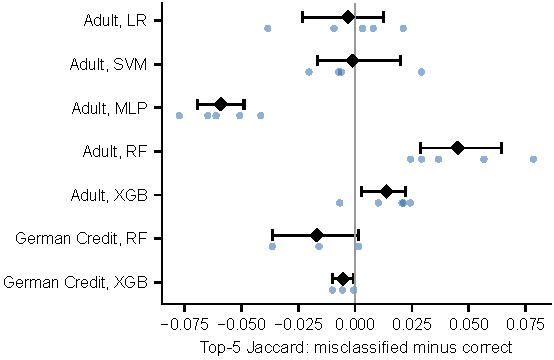
\includegraphics[width=\columnwidth]{figures/fig3_correctness.pdf}
\caption{Difference in top-5 overlap, misclassified minus correct. Points are seeds; diamonds are means with seed-clustered 95\% intervals (spread of the seed means)}
\label{fig:correctness}
\end{figure}

\subsection{Disagreement and Explanation Quality (RQ4)}

Table~\ref{tab:quality} and Fig.~\ref{fig:quality} give the within-run Spearman
correlation between disagreement and the four quality values. The clearest pattern
concerns the fidelity of LIME: on Adult the correlation was negative for all five model
families (from $-$0.45 to
$-$0.19), and it was negative on German Credit
($-$0.26 and
$-$0.24); on Breast Cancer it was negative for the
random forest ($-$0.28) and near zero for gradient
boosting. The two methods disagreed more on the
instances where the sizes of the LIME attributions followed less closely the effect of
masking each feature. The
correlations with the fidelity of SHAP were closer to zero and of mixed sign.

For stability there was no common pattern. On Adult the correlations were small and
mostly positive, except for the multilayer perceptron. For LIME on Adult they cannot be
interpreted: the stored stability of LIME has almost no range there (its median by model
lies between 0.001 and 0.009, against
0.793 to 0.865 on German Credit and
0.943 to 0.955 on Breast Cancer; post hoc). On
Breast Cancer, disagreement was higher for instances with less stable explanations of
either method, for the random forest ($-$0.56 and
$-$0.54) and less so for gradient boosting
($-$0.34 and $-$0.27),
with three runs each. These are associations within runs; they do not show that low fidelity
causes disagreement. The fidelity measure rewards attributions whose size follows the
effect of replacing a feature by its mean, which is a contribution; a vector of slopes is
at a disadvantage by construction, so part of this association may reflect how far the
slopes of an instance are from its contributions.

\begin{table}[t]
\renewcommand{\arraystretch}{\tablestretch}
\centering
\caption{Mean within-run Spearman correlation between disagreement ($1 - J_5$) and explanation quality. Fid.: fidelity; Stab.: stability. On Adult the stored LIME stability has almost no range, so the last column cannot be interpreted for that dataset}
\label{tab:quality}
\small
\setlength{\tabcolsep}{\mediumcolsep}
\begin{tabular}{llrrrr}
\hline
 & & \multicolumn{2}{c}{SHAP} & \multicolumn{2}{c}{LIME} \\
Dataset & Model & Fid. & Stab. & Fid. & Stab. \\
\hline
% GENERATED by scripts/build_paper_e.py -- do not edit
Adult & LR & $-$0.01 & 0.09 & $-$0.40 & 0.12 \\
 & SVM & $-$0.05 & 0.06 & $-$0.45 & 0.12 \\
 & MLP & $-$0.06 & $-$0.24 & $-$0.19 & $-$0.07 \\
 & RF & $-$0.22 & 0.23 & $-$0.27 & 0.10 \\
 & XGB & $-$0.15 & 0.14 & $-$0.40 & 0.11 \\
\hline
German Credit & RF & $-$0.05 & $-$0.06 & $-$0.26 & $-$0.10 \\
 & XGB & $-$0.04 & 0.02 & $-$0.24 & $-$0.15 \\
\hline
Breast Cancer & RF & $-$0.06 & $-$0.56 & $-$0.28 & $-$0.54 \\
 & XGB & 0.22 & $-$0.34 & 0.01 & $-$0.27 \\
\hline

\end{tabular}
\end{table}

\begin{figure*}[t]
\centering
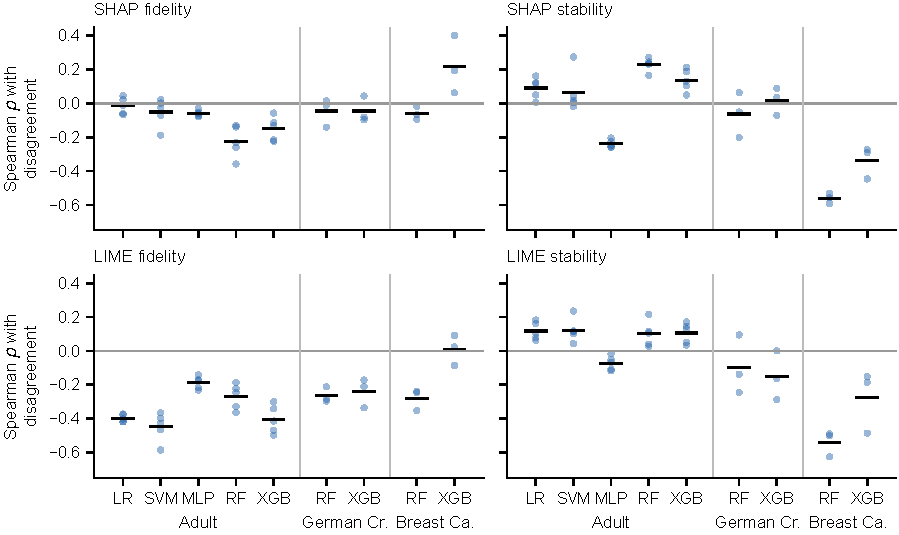
\includegraphics[width=\textwidth]{figures/fig4_quality.pdf}
\caption{Within-run Spearman correlation between disagreement and four quality values. Points are seeds; bars are means over seeds}
\label{fig:quality}
\end{figure*}

\subsection{Feature Sets of Anchors and DiCE (Secondary)}

Table~\ref{tab:secondary} gives the overlap between feature sets on Adult. The features
in an Anchors rule overlapped more with the SHAP top-5 set
(0.348) than with the LIME top-5 set
(0.240). The features changed by DiCE overlapped little with any
other set (at most 0.078). These methods answer different questions,
a sufficient condition and a minimal change, so a low overlap is not an error of either
method; it shows that their features cannot be substituted for those of an attribution
method.

\begin{table}[t]
\renewcommand{\arraystretch}{\tablestretch}
\centering
\caption{Jaccard overlap between feature sets on Adult (SHAP, LIME: top-5 features; Anchors: rule features; DiCE: changed features): mean of run means and seed-clustered 95\% interval (spread of the seed means)}
\label{tab:secondary}
\footnotesize
\setlength{\tabcolsep}{\tightcolsep}
\begin{tabular}{lrrrl}
\hline
Feature sets & Runs & Pairs & Mean & 95\% int. \\
\hline
% GENERATED by scripts/build_paper_e.py -- do not edit
SHAP vs. Anchors & 56 & 14,584 & 0.348 & [0.340, 0.356] \\
LIME vs. Anchors & 57 & 19,095 & 0.240 & [0.234, 0.247] \\
SHAP vs. DiCE & 67 & 25,248 & 0.078 & [0.068, 0.087] \\
LIME vs. DiCE & 68 & 29,830 & 0.078 & [0.074, 0.085] \\
Anchors vs. DiCE & 53 & 18,578 & 0.068 & [0.062, 0.075] \\
\hline

\end{tabular}
\end{table}

\section{Discussion}
\label{sec:discussion}

\textbf{The choice of explainer changes the explanation, and so does a second run.} On
two of the three datasets, SHAP and LIME shared on average fewer than three of their five
most important features. A user who reads a top-5 list would often see a different list
with the other method. This agrees with the disagreement reported by Krishna et al.
\cite{krishna2024disagreement}. The self-agreement experiment qualifies it: the user would
also see a partly different list from the same method with another random state. Disagreement between methods was larger than this within-method variability for
every model, so it is real, but a comparison of two explainers that ignores their
repeatability overstates how much they differ. For LIME, more perturbed samples would
raise the repeatability; the 1000 used here are fewer than the default of the package.

\textbf{Agreement varies with the model and the data.} The differences between models and
between datasets were larger than every other effect measured here. One reading is that
the methods approximate the model in different neighbourhoods \cite{han2022which} and
coincide more where the model is close to linear; another is that the repeatability of
the explainers itself changes with the model, as for the multilayer perceptron
(Table~\ref{tab:ceiling}). These data do not separate the two, and on Adult each family is a single
fitted model. The high overlap on Breast Cancer is mostly agreement on a ranking of the
features that is nearly the same for every instance; the overlap that depends on the
instance was small on the three datasets and smallest there. A high overlap is therefore
not evidence that two explainers agree about the individual prediction. A report of
explainer agreement should state the model, the dataset, the configuration and the
repeatability of each method and the overlap between explanations of different instances,
and should not be generalised from one of them.

\textbf{Signs need the same quantity.} The sign analysis shows a risk for any study that
compares the direction of attributions between methods. A LIME coefficient without
discretisation is a slope; a SHAP value is a contribution relative to a reference
\cite{garreau2020explaining,lundberg2017unified}. Their signs differed for almost every
instance of one class on Breast Cancer, while the two methods implied the same global
direction for the feature: after the slope was multiplied by the deviation of the feature
from the training mean, the signs agreed for more than nine shared features out of ten on
every dataset and model. Before signs are compared, the two explanations should be brought
to the same quantity in this way, or LIME should be used with discretisation, whose
weights refer to the value of the instance. Roy et al. \cite{roy2022why} also found sign
disagreement to be the smaller part of the problem. In these data, the disagreement
between SHAP and LIME concerns which features are ranked first; on the direction of the
features they share, the two methods give no evidence of conflict, although a fixed
direction per feature would give the same agreement. The measures of overlap and rank used for RQ1 to RQ4 depend on absolute values and
are not affected by this difference of sign. A slope and a contribution also differ in
size, but re-ordering the LIME lists by contribution changed the overlap little.

\textbf{Disagreement and correctness.} Agreement was
not consistently lower when the model was wrong. The direction depended on the model, also
on held-out instances, and the differences were small. No consistent association between
disagreement and a wrong prediction was found in these data.

\textbf{Disagreement and LIME fidelity.} On Adult and, more weakly, on German Credit, disagreement was higher where the
fidelity of the LIME explanation was lower, that is, where the sizes of its attributions
followed the single-feature masking effects less closely. Since that measure favours
contributions over slopes, the association may indicate the instances where the slope and
the contribution of LIME differ most. It is an association within runs, on a proxy
measure.

\textbf{Limitations.} The study covers three tabular binary datasets and one
configuration of each explainer. LIME was used with a kernel width of 3, chosen
without a technical reason and smaller than the default of the package.
With this width the 999 perturbed samples of an explanation, drawn around the training
mean, together receive a median weight of 0.26 on Adult,
2.3 on German Credit and 83.6 on Breast Cancer,
against a weight of one for the instance itself (post hoc), and the stored stability of
LIME on Adult is close to zero. Section~\ref{sec:results:ceiling} shows how much the
width changes the LIME lists; other sample sizes or discretisation settings may change the
estimates as well. There are five seeds on Adult and three on
the other datasets; the intervals describe the spread of seed means and the analyses of
RQ2 to RQ4 are exploratory. On Adult each model family is one fitted model, so nothing
here separates a family from that fit. The self-agreement experiment used a small
subsample and one pair of random states. Only the ten largest features of each explanation were stored, which limits
the rank measure to that list. One-hot columns were treated as separate features; an
analysis by original variable would give higher overlap. Fidelity and stability are proxy measures computed without ground-truth explanations. On
Adult, each model was trained once, and for four of the five seeds about seven in ten of
the explained instances belong to its training data; the mean top-5 overlap for seed 42,
whose evaluation partition is disjoint from the training data, lies within the range of
the other four seeds, and the correctness contrast was repeated on held-out instances.
LIME, as configured, also treats one-hot columns as continuous, so its slopes are only
loosely local. The conversion of slopes into contributions uses the training mean as reference,
while SHAP uses the expected output on a background sample, so the two references are
close but not identical. The SHAP runs of the SVM are incomplete, so that family has fewer pairs, unevenly
distributed between the predicted classes. The models of the two smaller datasets were regenerated from the training recipe
and validated against stored metrics and predictions, not compared byte by byte with the
original binaries. For the Adult random forest, the stored binary does not reproduce all
the predictions recorded in the runs; the agreement analyses use only the recorded
outputs, and the paired SHAP and LIME records agree on every label and prediction. The
self-agreement experiment, which needs the binary, kept only the instances whose recorded
prediction it reproduces. The sign analysis,
including the conversion into contributions, is post hoc.

\section{Conclusions and Future Work}
\label{sec:conclusions}

For the same instance and model, SHAP and LIME agreed only partly on the most important
features: the mean top-5 overlap was 0.393 on Adult,
0.387 on German Credit and
0.714 on Breast Cancer. Much of this overlap, and
most of it on Breast Cancer, was also found between explanations of different instances,
so it reflects a ranking of the features common to the instances; the part specific to
the instance was 0.191 on Adult and smaller on the other two
datasets (post hoc). Each method also agreed only
partly with itself when run again, and the agreement between the methods was below that
self-agreement for every model tested (post hoc). Agreement varied with the model and the
dataset, not visibly with the number of explained instances, and it was not consistently
lower for misclassified instances. The sign agreement between SHAP and LIME without
discretisation followed the predicted class, because one method returns slopes and the
other contributions (post hoc). After conversion to contributions the signs of the shared
top features agreed in 0.945 to
0.990 of the cases, the level that one fixed direction per
feature reaches. Sign agreement should not be used as a measure of disagreement unless
both explanations are first expressed as the same quantity.

Three practical consequences follow. An explanation shown to a user should name the
explainer, since another explainer would often show other features. A comparison of
explainers should report how well each one reproduces itself and how much two explanations
of different instances overlap, since these set the levels against which their agreement
can be judged. And it should check, before any measure
is computed, what each stored value means.

Future work will measure self-agreement on the full cohort, with more LIME samples and
with other kernel widths,
compare the methods on a common quantity, repeat the analysis by original variable, and
add models and datasets to separate the effect of the model family from that of a single
fit.

\section*{Data Availability}
\iffull
The three datasets are public
\cite{becker1996adult,hofmann1994statlog,wolberg1993breast}. The code, the per-instance
run outputs, the new LIME cohort, the pre-specified analysis plan and every result file are
available at \url{https://github.com/jonnabio/xai-eval-framework} (release
\texttt{\papererelease}), archived at \paperearchive. Every number, table
and figure in this article is generated from those files by the scripts described in
\texttt{docs/reports/paper\_e/README.md}.
\else
The three datasets are public
\cite{becker1996adult,hofmann1994statlog,wolberg1993breast}. The code, the per-instance
run outputs, the new LIME cohort, the pre-specified analysis plan and every result file are
in a public repository, with scripts that generate every number, table and figure in
this article; its address is withheld for blind review.
\fi

% cys.bst prints a DOI as \url{10.xxxx/...}, which is not an address. Inside the reference
% list a DOI therefore links to https://doi.org/<doi>, and complete addresses in the .bib
% file use \fullurl.
\let\fullurl\url
{
\renewcommand{\url}[1]{\href{https://doi.org/#1}{\nolinkurl{#1}}}
\bibliographystyle{cys}
\bibliography{references}
}

% Journal footer, as in the CyS template (example.tex). The journal fills in the dates,
% which it prints day first (its example reads "accepted on 16/01/2017").
{\vskip 12pt}
\noindent
\footnotesize {\textit{Article received on DD/MM/YYYY; accepted on DD/MM/YYYY.\iffull\\
{*}Corresponding author is Jonathan Herrera-V\'asquez.\fi}}

\end{document}
